% vim: ts=2:sw=2:tw=80:et
\thispagestyle{fancy}
\pagestyle{fancy}

The primary use of Arbwave is to create a coordinated, arbitrary, multi-channel
waveform using a multitude of voltages, currents, frequeny sources, digital
signals, or other experimental controls.  The interface in Arbwave is geared
towards making arbitrary waveforms as simple as possible while still allowing
very complex waveform features.  This chapter describes the techniques used in
Arbwave to define the waveforms.  The first section discusses some basic
concepts used in all components of the waveform.  The next three sections discuss
how to create waveform components, with increasing levels of complexity covered.

\section{Basic Concepts}
\begin{figure}[ht!]
  \centerline{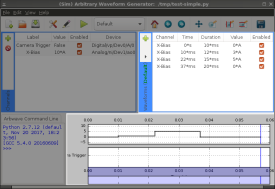
\includegraphics[width=.8\textwidth]{figures/basic-waveform}}
  \caption[Very simple waveform]{
    A very simple waveform of one channel with explicitly set times and
    durations.  The bottom of the highlighted portion, shows how the analog
    \textbf{X-Bias} channel varies over time.
  }
  \label{fig:waveforms:basic}
\end{figure}

The fundamental component of a waveform is a \textit{Waveform Element}.  The
\textit{Waveform Element} identifies a single output channel, a timeframe for
the \textit{Waveform Element}, and a value of the output channel for the given
timeframe.  Thus, each \textit{Waveform Element} represents a single (or set of)
transition(s)--a transition being any intentional change or reprogramming of the
output value of a channel.

A waveform consists of one or more transitions, as defined by a sequence of
\textit{Waveform Element}s, that are coordinated in time such that their
occurrence is deterministic.  \textit{Waveform Element}s are added/deleted using
the buttons on the left side of the \textit{Waveforms} section of the main
window--the top of the highlighted area in Fig.~\ref{fig:waveforms:basic}.  Once
added, \textit{Waveform Element}s can be rearranged using drag-drop maneuvers.
Additionally, \textit{Waveform Elements} can be copied using the
\textbf{Control} key while dragging \textit{Waveform Element}s.

As an example of a simple waveform and sequence of transitions, consider the
configuration created
in Chaps.~\ref{chap:devcfg} and~\ref{chap:channels}.  Continuing this example,
one can use the \textit{Waveform} section of the main window to define an
arbitrary set of transitions.  For instance, a simple waveform representing four
sequential steps of the \textbf{X-Bias} current can easily be created, as
represented in the highlighted portion of Fig.~\ref{fig:waveforms:basic}.  As
shown, each \textit{Waveform Element} (or row in the \textit{Waveforms} section)
has an associated output channel, a beginning time, a duration, a constant
value, and a flag that indicates whether the element should be enabled.

As a waveform is built, Arbwave ensures that each transition occurs exactly in
accordance to the timing of the device clock source (see
Chap.~\ref{chap:devcfg}).  Using this precise time information, Arbwave shows
the analog and digital waveforms that should be generated in waveform-plot
viewport--the reader should easily note this Arbwave waveform plotting facility,
as shown in the bottom of the highlighted portion of
Fig.~\ref{fig:waveforms:basic}.

Although Fig.~\ref{fig:waveforms:basic} explicitly specifies absolute start time
and duration of the \textit{Waveform Element}s, it is often much more
advantagous to specify these in relative mode, taking advantage of Arbwave's
ability to automatically calculate the actual time of a \textit{Waveform
Element}.  Furthermore, it is often desirable to specify the value of a channel
in a manner that (at least somewhat) smoothly varies the channel over the
duration of \textit{Waveform Element}.  Both of these concepts are discussed in
more depth in Secs.~\ref{sec:waveforms:nattime} and~\ref{sec:waveforms:value}
respectively.  Furthermore, more complicated waveforms using hierarchical groups
will be discussed in Sec.~\ref{sec:waveforms:groups}.



\subsection{Automatic Waveform-Element Variables}\label{sec:waveforms:vars}

In order to help ease the creation of more complex waveforms, Arbwave automatically 
defines a few variables for the user.  These variables represent various
useful quantities such as current start time of a waveform component, taking
into account all \textit{Waveform Element}s that have gone before, and also
another representing the value of a particular channel as it settled before the
current \textit{Waveform Element}.  The various automatically-defined variables
are listed in Tab.~\ref{tab:waveforms:autovars}.  The meaning and use of these
variables will become more clear through the remainder of this chapter.

\begin{table}[htb!]
\begin{center}
  \begin{tabular}{|L{1.5cm}|c|C{1cm}|C{2cm}|C{2cm}|C{2cm}|}
    \hline
    Variable Name  & Description  & Group Scope & Waveform Element Scope
                   & \hyperref[sec:waveforms:expr]{Value Expressions}
                   & \hyperref[sec:waveforms:generators]{Value Generators}\\
    \hline
    \symb{natural_time} & Currently progressed natural time & X & X & X & X\\
    \symb{duration}     & Duration of current group         & X & X & X & X\\
    \symb{dt_clk}       & Minimum clock period of channel   &   & X & X & X\\
    \symb{U0}           & Last value of channel             &   & X & X & X\\
    \symb{relative_time}& Relative waveform-element time    &   & X & X &  \\
   \hline
  \end{tabular}
  \caption[Automatic waveform variables]{
    \label{tab:waveforms:autovars}
    Automatically defined waveform variables allow natural and easy entry of
    waveform elements.
  }
\end{center}
\end{table}




\section{Natural Time}\label{sec:waveforms:nattime}

\begin{figure}[ht!]
  \centerline{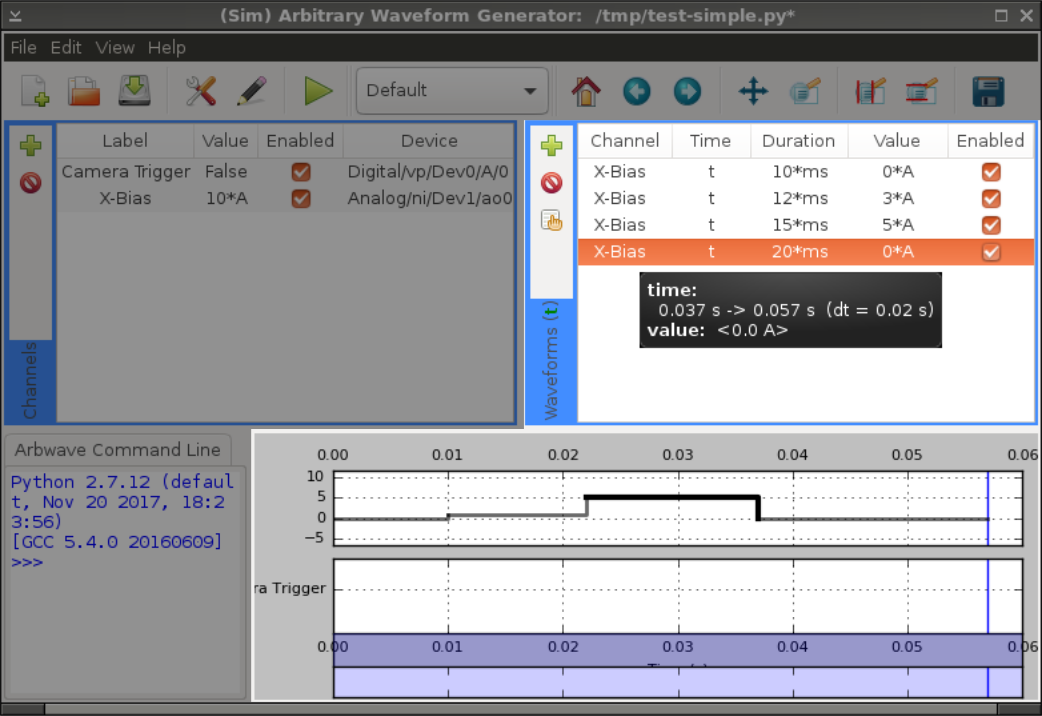
\includegraphics[width=.8\textwidth]{figures/basic-waveform_t}}
  \caption[Very simple waveform using \textit{Natural Time} \symb{natural_time}]{
    A very simple waveform of one channel with explicit durations but using
    \textit{Natural Time} to indicate the start of each \textit{Waveform
    Element}.  Note that highlighting a \textit{Waveform Element} shows a popup
    with the final-computed time of the \textit{Waveform Element}.
  }
  \label{fig:waveforms:basic_t}
\end{figure}

One of the first automatically generated variables that a user becomes
acquainted with is denoted \symb{natural_time}.  As shown in
Tab.~\ref{tab:waveforms:autovars}, the definition of this variable is not simply
time, but rather the \textit{Natural Time} to start a \textit{Waveform Element}
or group of elements, based on what has preceded.  Generally, this time
corresponds with the time that all previous \textit{Waveform Elements} have
completed their prescribed changes, ignoring any \textit{Waveform Elements} which
have been set to be Asynchronous (which can be done by right clicking on a 
\textit{Waveform Element} and checking the box that appears.  Consider the earlier waveform
shown in Fig.~\ref{fig:waveforms:basic}.  Instead of specifying the start time
of each \textit{Waveform Element} explicitly in absolute time (with respect to
the start of the waveform), we could choose to instead allow Arbwave to
calculate the correct start time for each of the \textit{Waveform Elements}.  By
specifying the start time as \textit{Natural Time} \symb{natural_time}, we get
the same waveform, but without the need to calculate the actual start time of
each \textit{Waveform Element}--this is shown in
Fig.~\ref{fig:waveforms:basic_t}.

Just as in any other input in Arbwave, the expression that is put into
the \textit{Time} column for a \textit{Waveform Element} may be any Python
expression that evaluates to a value with units of time.  Thus, it is possible
to offset the \textit{Natural Time} \symb{natural_time} with any other time
expression.  It is even possible to put the time of one \textit{Waveform Element} in absolute
form (such as in Fig.~\ref{fig:waveforms:basic}) while others use the
automatically calculated \textit{Natural Time} \symb{natural_time}.

Finally, in specifying the times and durations of various \textit{Waveform
Element}s, one should be aware that \textit{Waveform Element}s of any single
output channel \underline{cannot} overlap in time with any other
\textit{Waveform Elements} of the same channel.  Arbwave does take care to test
all \textit{Waveform Elements} for overlap with others from the same channel.
If such overlapping \textit{Waveform Elements} are detected, an error is emitted
and the waveform processing is halted.  In such a case, the user must correct
the situation before Arbwave will successfully complete the next waveform
generation.



\section{Waveform Element-Values}\label{sec:waveforms:value}

The value of each waveform element, in the most basic form, may be specified as
a single value with units appropriate for the respective channel.
%
Often times, a single value for a waveform element is not sufficient.  Arbwave
provides two mechanisms that allow a single waveform element to represent a
time-varying function.  The simplest of these two is using \textit{Value
Expressions}.  The second mechanism is using the much more powerful, extensible,
but much more complicated-to-extend \textit{Value Generators}.  These two
mechanisms areas discussed in the following Sec.~\ref{sec:waveforms:expr} and
Sec.~\ref{sec:waveforms:generators} respectively.


\subsection{Value Expressions}\label{sec:waveforms:expr}
\textit{Value Expressions} provide a fairly simple mechanism to have a single
waveform element represent a larger time-varying function.  \textit{Value
Expressions} rely on the Python SymPy package being installed.  From the SymPy
webpage~\cite{sympy}:
\begin{quote}
SymPy is a Python library for symbolic computation. It provides computer algebra
capabilities either as a standalone application, as a library to other
applications\ldots
\end{quote}
After Arbwave successfully automatically tests if the SymPy package is
available, the \textit{Value Expressions} interface is enabled and the user may
specify functional forms of values for a waveform element.

\subsubsection{Basics}

When using expressions, in
order to define how a channel's value should change over time, one uses the
symbol \symb{relative_time} to represent relative waveform-element time.
\symb{relative_time} always varies
from 0 to 1.  Thus, for a waveform element with duration \symb{duration},
\symb{relative_time} varies from 0 to 1
over the duration of the waveform element.

As an example of using expressions, consider the \op{Ramp} value generator
function.  This function generally varies the channel as:
%
\begin{lstlisting}
  U0 + (U1 - U0)*x**E
\end{lstlisting}
%
where U0 and U1 are the beginning and ending values of the ramp respectively and
E is the power of the time dependence.  If, for instance, a voltage channel
required to be changed from its original value to a final value of 10*V with a
square-root time dependence, one could simply use an expression like:
%
\begin{lstlisting}
  U0 + (10*V - U0)*x**0.5
\end{lstlisting}
%
Using expressions, it is much simpler for the user to specify somewhat arbitrary
functional forms of waveform values.  For instance, one can specify an Gaussian
change function as something like:
%
\begin{lstlisting}
  10*V * sy.exp(-(x-.5)**2.0 / (2 * .1**2.0))
\end{lstlisting}
%
where sy represents the sympy module as imported in the global script as:
\begin{lstlisting}
  import sympy as sy
\end{lstlisting}

\subsubsection{Value Expressions Advanced}
Just as many \textit{Value Generators} allow the user to use functional arguments to
modify the waveform generated, such as the number of steps in a \op{Ramp},
\textit{Value Expressions} similarly provides a method to modify the output.
%
There are three primary parameters to modify the resulting waveform of an
expression:
\begin{itemize}
  \item \var{expr\_fmt}
    \begin{itemize}
    \item uniform\\
      Causes the output waveform to be uniformly discretized in time.
    \item optimize\\
      Causes the output waveform to be optimally discretized in time such that a
      constant total err (\var{expr\_err}) is maintained for each linear
      time segment.
    \end{itemize}
  \item \var{expr\_steps}\\
    Influences the number of (possible) steps used in evaluating \textit{Value
    Expressions}.  The exact meaning of \var{expr\_steps} depends on the value of
    \var{expr\_fmt}:
    \begin{itemize}
      \item $\var{expr\_fmt} = \op{uniform}$:\\
        \var{expr\_steps} sets the number of fixed-size steps to make over the duration.
      \item $\var{expr\_fmt} = \op{optimize}$:\\
        \var{1/expr\_steps} defines the minimal relative time-step to consider
        when creating a line segment that such that error along the line is
        estimated to be $\le \var{expr\_err}$.
    \end{itemize}
  \item \var{expr\_err}\\
      See $\var{expr\_fmt} = \op{optimize}$ above.
\end{itemize}
%
There are three possible methods to set each of these \textit{Value Expression}
parameters:
\begin{itemize}
  \item globally (i.e. in embedded Python shell or in global script)
  \item local to group (in a local group script)
  \item local to waveform element:\\
    If one desires the scope of these parameters to be limited to a single
    element, one must wrap the expression by the \op{expr} function.
    The signature to this function is given by:\\
      \op{expr(expression, steps=None, err=None, fmt=None)}
\end{itemize}



\subsection{Value Generators}\label{sec:waveforms:generators}
Value generators allow more power waveform generation control for a single
waveform element.  Rather than simply expressing the functional form of the
waveform element, a value generator instantiates the respective value-generator
class, which is then responsible for returning an iterator of waveform points
back to arbwave.
%
\begin{lstlisting}
class ValueGenerator(object):
  # Arbwave uses this string to represent the generator to the user.  It must be
  # a valid Python identifier, but may be something different than the exact
  # spelling (including case) of the generator class.
  name = 'valueGenerator'

  def __init__(self, arg0, arg1, arg2):
    """
    Usage:  valueGenerator(arg0, arg1, arg2)

    When the user creates the generator using the Python identifier from
    self.name, this is the constructor called (i.e. the signature of the
    generator).  The various arguments depend on the generator's use and may
    include default values.

    ***The documentation provided here is shown to the user in the \textit{Value
    Generators} help menu.***
    """
    super(ValueGenerator, self).__init__()
    ...

  def set_vars(self, _from, t, duration, dt_clk):
    """
    Arbwave uses this function to give channel-specific information to the
    generator.
      _from : is the last value (with units) of this channel before this
              waveform element
      t     : is the absolute start time of the waveform element ***in integer
              units of dt_clk***
      dt    : is the duration of the waveform element ***in integer units of
              dt_clk***
      dt_clk: is the duration of the clock pulse that is used for this channel
              in proper units (seconds)
    """
    pass

  def set_units(self, units, units_str):
    """
    Arbwave calls this function if it exists to give the generator the
    user-specified units and units string for the particular channel.
    """
    pass

  def get_encoding(self, capabilities):
    """
    Given the set of capabilities supported by the channel, this function
    returns the encoding desired.
    """
    pass

  def __repr__(self):
    """
    Show return a string that correctly represents the constructor of the
    generator as used by the user.  This will be used in tooltips to show the
    value of the waveform element.
    """
    pass

  def __iter__(self):
    """
    Must return an iterator that runs over the generated waveform.

    Each value returned by this iterator must be a tuple such as:
    (t, dt, v)
    where t and dt are the start time and duration of the waveform component
    ***in units of dt_clk*** for the channel respectively and v is the value
    (with the correct units for the channel).
    """
    pass

\end{lstlisting}
%
Currently, several value generators are supplied directly by Arbwave:
\begin{itemize}

\item \op{sinpulse}
\begin{lstlisting}
"""
    Usage:  sinpulse(A, F, average=0., phase_shift=0., steps_per_cycle=None):

    A       : Amplitude (0-to-peak)
    F       : Frequency in Hz
    average : Average value of sine wave.
    phase_shift : 0 to 2 pi shift, where pi/2 represents +cos
    steps_per_cycle   : number of steps per cycle

    Only one of dt or steps can be used.
"""
\end{lstlisting}

\item \op{ramp}
\begin{lstlisting}
"""
Usage:  ramp(to, exponent=1.0, steps=20, _from=None, dt=None, duration=None)

to      : final value to which to ramp
_from   : initial value from which to ramp
exponent: exponent with which to ramp
steps   : number of steps to take
dt      : the timestep to increment (Default: duration/steps)
duration: Duration of ramp function.  Note that this is not necessarily
          equal to the actual duration of the steps generated by the ramp,
          since those are set in the "Duration" field of the waveform
          editor.  Value of None indicates that the ramp should last for the
          time specified in the "Duration" field of the waveform editor.
          [Default: None]

Only one of dt or steps can be used.
"""
\end{lstlisting}

\item \op{pulse}
\begin{lstlisting}
"""
Usage:  pulse(high=True, low=None)

high  : The value to generate for the pulse.
low   : The value to return to after the pulse.
        If low is not set (left as None) it will be set differently for
        analog and digital channels.  If the high is a boolean value, low
        will be set to its logical complement.  Otherwise, if low is not
        set, it will be set to whatever the channel is at prior to this
        pulse.
"""
\end{lstlisting}

\item \op{pulses}
\begin{lstlisting}
"""
Usage:  pulses(n, duty=0.5, high=True, low=False, dt=None)

n     : Number of evenly spaced pulses to generate.
duty  : Duty cycle (only used if dt is not set) [Default 0.5].
high  : The value to generate for each pulses [Default:  True].
low   : The value to return to after the pulse.
        If low is not set (left as None) it will be set differently for
        analog and digital channels.  If the high is a boolean value, low
        will be set to its logical complement.  Otherwise, if low is not
        set, it will be set to whatever the channel is at prior to this
        pulse.
"""
\end{lstlisting}

\item \op{interp}
\begin{lstlisting}
"""
Usage:  interp(x, y, steps=20, dt=None)

x       : time in arbitrary units.  Time will be normalized to 0-1 where
          time=1 corresponds to the maximum value in x.
y       : y values to use in interpolation
steps   : number of steps to take (Default: 20)
dt      : the timestep to increment (Default: duration/steps)

Only one of dt or steps can be used.
"""
\end{lstlisting}
\end{itemize}


\section{Groups}\label{sec:waveforms:groups}

More complicated waveforms can be achieved by creating a hierarchical set of
groups and subgroups of \textit{Waveform Element}s.  This is done by performing
a grouping operation where dragging one \textit{Waveform Element} onto another
promotes the second to acting as a \textit{Group Element}.  Because
\textit{Group Element}s are not tied to any specific output channels,
\textit{Group Element}s do not have any value associated with them.
Additionally, the label of a \textit{Group Element} is not taken from a list of
channel names, but rather should be edited by the user to reflect something
meaningful for the group.

\subsection{Natural Time with Groups}
\textit{Natural Time} for groups is calculated slightly differently than for
\textit{Waveform Element}s.  While only preceding \textit{Waveform Elements} in
the same group (or at the root level of the hierarchy) of the same channel
affect \textit{Natural Time} of subsequent \textit{Waveform Element}s, all groups of
the same hierarchical level affect subsequent groups.  Furthermore, no
\textit{Waveform Element}s affect the calculation of \textit{Natural Time}.

For the \textit{Waveform Element}s or groups within a group, \textit{Natural
Time} is relative to the beginning of the group.  Thus, if the start time of the
\textit{Group Element} is modified, all children of the group move in time by
the same amount and direction.  This feature provides a very simple means to
move an entire subsection of the experimental output waveform from one timeframe
to another.

\subsection{Duration Inheritance}

\begin{figure}[hbt!]
  \centerline{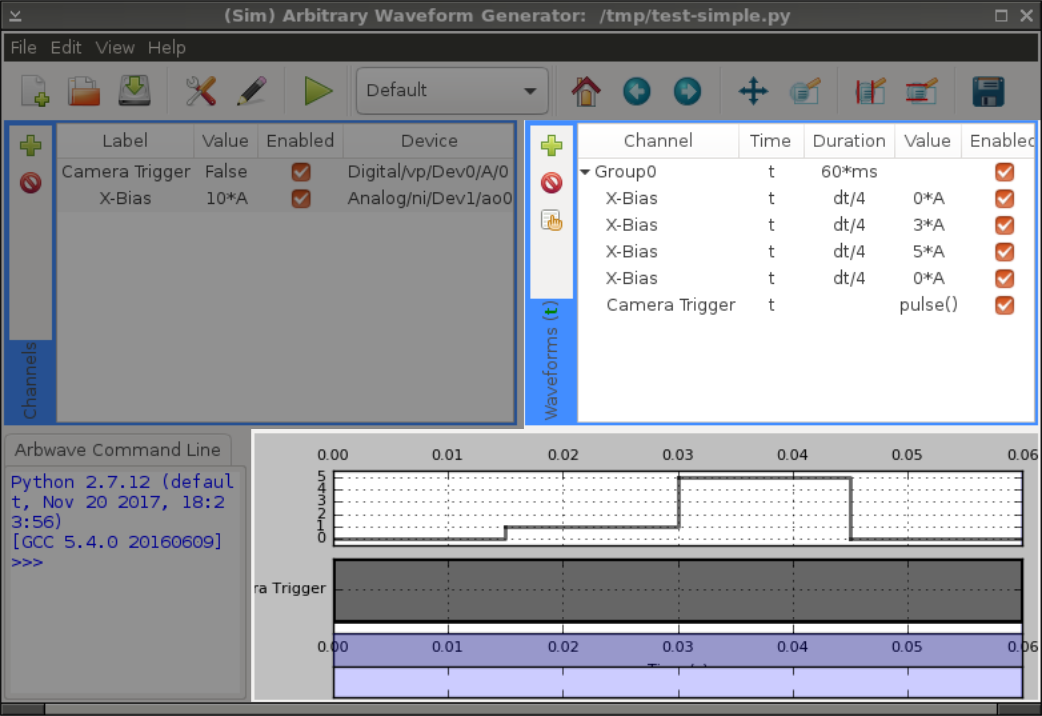
\includegraphics[width=.8\textwidth]{figures/basic-waveform_group}}
  \caption{
    Waveform demonstrating duration \symb{duration} inherited from the
    \textit{Group Element}
  }
  \label{fig:waveforms:basic_group}
\end{figure}

In Sec.~\ref{sec:waveforms:vars}, the notion of automatic variables is
introduced.  One of these variables is \symb{duration}, described there as
\textit{duration of current group}.  This variable is automatically provided to
all children of a group with the value being the duration of the \textit{Group
Element}.  Fig.~\ref{fig:waveforms:basic_group} shows our previous example
modified such that each of the \textit{Waveform Element}s belongs to the same
group and inherits its duration information from the \textit{Group Element}.
For the \textit{Waveform Element}s of the \textbf{X-Bias} channel, each duration
is calculated as a fraction of the duration of the \textit{Group Element}.

Instead of specifying some fraction (or all) of the \textit{Group Element}
duration, one can also simply omit the duration field---in this case, the
duration will automatically be set to the full duration of the parent
\textit{Group Element}.  As also shown in Fig.~\ref{fig:waveforms:basic_group},
this is demonstrated in the last \textit{Waveform Element} where the output
channel \textbf{Camera Trigger} is pulsed on for the entire duration of the
\textit{Group Element}.



\section{Waveform Selector}
Very often, when defining a very complicated experimental configuration, it can
be desirable to create and execute a very simple different waveform without
changing any of the device or channel configuration.  This is possible using the
\textbf{Waveform Set Editor}.  Selecting different defined waveforms and access
to the \textbf{Waveform Set Editor} is done by using the ``editor'' button just
below the \textbf{Delete Waveform Element} button.  One can also select or edit
waveforms using the context menu within the \textit{Waveform} section of the
main window.  The insert key is particularly helpful do create blank new waveforms.


\section{Execution}
When the entire waveform has been defined (and hence shown in the plot
viewport), one is ready to begin excuting the waveform.  The next chapters
discuss simple and also more complex methods of executing the waveforms.
